\documentclass{article}
\author{Dominic Yang}
\title{On the Computation of Master Corner Polyhedra}
\date{\today}

\usepackage{amsmath}
\usepackage{amssymb}
\usepackage{amsthm}
\usepackage{algorithm}
\usepackage{algpseudocode}
\usepackage{booktabs}
\usepackage{graphicx}

\newtheorem{theorem}{Theorem}
\newtheorem{corollary}{Corollary}

\begin{document}
	\maketitle

	\section{Abstract}
	In this report, we report on the computational difficulties in the enumeration of the Master Corner Polyhedra arising from Gomory's corner relaxation. We develop the notion of the corner polyhedron and its connection with cutting planes and then motivate the construction of the master corner polyhedron as an all-encompassing polyhedron of which other corner polyhedra are subsections of. We then compare Gomory's original linear programming formulation for the master polyhedra and analyze its efficacy for the enumeration of the polyhedra and discuss alternative formulations for the computation of such objects.

	\section{Introduction}
	
	Mixed integer optimization programs cover an extremely broad class of problems ranging from classic combinatorial optimization problems such as the traveling salesman problem to questions of scheduling in the context of operations research or the determination of the optimal placement of facilities. These problems are generally framed in the following (or an equivalent) form
	\begin{equation*}
	\begin{aligned}
	& & & \text{minimize } c^T x \\
	& & & \text{subject to} \\
	& & & Ax = b \\
	& & & x_j \in \mathbb{Z}, j=1,\ldots,p \\
	& & & x_j \ge 0, j=1,\ldots,n \\
	\end{aligned}
	\end{equation*}
	where $p \le n$, $A \in \mathbb{R}^{m \times n}$ is a matrix of full row rank, and $b \in \mathbb{R}^m$. 
	
	In accordance with the procedure delineated in the simplex algorithm, we can write the above system using basic and nonbasic variables. Given a feasible basis $B \subset \{1,\ldots,n\}$ and nonbasic variables indexed by $N = \{1,\ldots,n\} \ B$, we can write the system as
	\begin{equation}
		x_i = \bar{b_i} - \sum_{j \in N}\bar{a_{ij}}x_j, i \in B
	\end{equation}

	Of particular interest when studying these programs is the underlying geometry behind a given mixed integer program and how one may utilize this geometry to find optimal solutions to a program. When working with the underlying polyhedron of the integer program, one wishes to find cutting planes which will separate the fractional vertices which will be determined to be optimal on the linear programming relaxations of an integer program. 
	
	
	Some traditional cutting plane algorithms include Gomory's fractional cut which is determined by a single row of the simplex tableau $i$ with fractional value and is given by
	\begin{equation}
		\sum_{j \in N} f_{ij}x_j \ge f_i
	\end{equation}
	where $f_{ij} = \bar{a}_{ij} - \lfloor \bar{a}_{ij} \rfloor$ and $f_{i} = \bar{d}_i - \lfloor \bar{d}_i \rfloor$. 
	The Dantzig Cut is a separate cutting plane given by
	\begin{equation}
		\sum_{j \in N}x_j \ge 1
	\end{equation}
	A stronger cutting plane is given by Gomory's Mixed Integer Cut (GMIC) which is defined by the equation
	\begin{equation}
		\sum_{j \in N} \min\left\{\frac{f_{ij}}{f_i}, \frac{1 - f_{ij}}{1 - f_i} \right\}x_j \ge 1
	\end{equation}
	
	One observation which was made by Philippe, Richard, and Dey in \cite{jean50group} is that none of these cutting planes have any dependencies on the nonnegativity of the basis variables. This brings up the question of whether we could then for a given basis $B$, we could relax the constraints on nonnegativity and study the cutting plane algorithms that are valid on this new polyhedron. Then any cutting planes valid for this larger polyhedron will be valid for the polyhedron on our original problem.
	
	In constructing the corner polyhedron for a given basis $B$, we relax the constraints that basis variables be nonnegative. Note that relaxing nonnegativity constraints for a real variable $x_i$ in the basis leaves just the constraint $x_i = \bar{b_i} - \sum_{j \in N} \bar{a}_{ij}x_j$ which will be automatically satisfied meaning we can discard it. From here on, we shall then assume that all variables in the basis are integer variables.
	Under this scheme, we have the following equations describing the corner relaxation written in simplex tableau form:
	\begin{equation}
	\begin{aligned}
	& & & x_i = \bar{b}_i - \sum_{j\in N} \hat{a}_{ij}x_j, i \in B \\
	& & & x_i \in \mathbb{Z}, i=1,\ldots,p \\
	& & & x_j \ge 0, j \in N \\
	\end{aligned}
	\end{equation}
	We can reframe the first equality in the form
	\begin{equation}
		\bar{b}_i \equiv \sum_{j \in N} \hat{a}_{ij}x_j (\text{mod } 1) ,i \in B 
	\end{equation}
	or in matrix form
	\begin{equation}
		b \equiv Nx_N (\text{mod } B)
		\label{group_relation}
	\end{equation}
	where $x_N$ is a collection of integer vectors, $B$ is the submatrix with columns corresponding to basis variables, and $N$ the submatrix with columns corresponding to nonbasis variables, and the modulus of $B$ is understood to mean that $b$ differs from $Nx_N$ by some combination of basis vectors.

	The convex hull of the integer solutions to these points is referred to as the \textbf{Corner Polyhedron}. These geometric structures were first discussed by Gomory and expanded upon in a series of papers \cite{gomory1969some}. They have found use for the construction of cutting plane algorithms in the form of intersection cuts \cite{conforti2011corner}. 

	\section{Gomory's Master Polyhedra}
	In light of (\ref{group_relation}) which exposes the group theoretic underpinnings behind the corner polyhedron, we can ask further questions about how the corner polyhedron reveals itself when examined in the space of the nonbasic variables. In this exposition, we mostly follow Gomory in his classic paper \cite{gomory1969some}. If we let $f$ denote the homomorphism from $\mathbb{R}^m$ to $I^m$ given by taking the fractional part of each component, then we can apply $f$ to tp (\ref{group_relation}). Letting $N_i$ denote the $i$th column of $N$, we have that $f(b) = \sum_{i \in N}f(N_i)x_i$.
	Letting $f(b) = g_0$ and $f(N_i) = g_i$, we have the group equation
	\begin{equation}
		\sum_{i \in N}g_ix_i = g_0
	\end{equation}
	The integers $x_i$ which satisfy this equation correspond to integer points of the corner polyhedron in the original space of variables. In general $f$ is not an injection from the set of column vectors to group elements, so we introduce a new set of elements $g \in \mathcal{N}$ corresponding to unique group elements mapped onto by $f$ and $t_g$ which will be the sum of $x_j$ where $f(N_j) = g$. Then in this new space of variables, we have
	\begin{equation}
		\sum_{g \in \mathcal{N}}gt_g = g_0	
		\label{groupsum}
	\end{equation}
	
	Gomory denotes this polyhedron as $P(G, \mathcal{N}, g_0)$ where $G$ denotes the group, and $\mathcal{N}$ denotes the actual subgroup of interest in (\ref{groupsum}). The corresponding polyhedron in the original space of variables is referred to as $G_x(B, N, b)$. These two polyhedra can be shown have certain features in direct correspondence; in particular, Gomory demonstrates that vertices and faces of the two polyhedra are in bijection with each other \cite{gomory1969some}.
	
	An immediate question worth answering is how to characterize these polyhedra in the space that they live in. Specifically, we are interested in the faces of the polyhedra, if $(\pi, \pi_0)$ is a cutting plane with $\pi \in \mathbb{R}^{|\mathcal{N}|}$ should that for all integer points $t$ in $P(G, \mathcal{N}, g_0)$, we have that $\pi t \le \pi_0$, what constraints does that put on the possible values for $\pi$?
	If $\pi_0 = 0$, we have the following answer from Gomory \cite{gomory1969some}
	\begin{theorem}
		If $(\pi, 0)$ is a face of $P(G, \mathcal{N}, g_0)$, then we have that $\pi = e_g$, the vector with $t_g = 1$ and $t_h = 0$ for $h \not= g$. 
	\end{theorem}
	This tells us immediately that the faces with $\pi_0 = 0$ are the $\mathcal{N}$ hyperplanes orthogonal to the canonical unit vectors and contain the origin.
	This gives us a characterization of these faces.
	
	The faces with $\pi_0 > 0$ for these polyhedra are a fair bit more complicated. We introduce the master corner polyhedron to discuss this notion. We define the \textbf{Master Corner Polyhedron} as $P(G, G_+, g_0)$ where $G_+ = G/\{0\}$. It can be shown that any for any $\mathcal{N} \in G_+$, we can compute $P(G, \mathcal{N}, g_0) = P(G, g_0) = E(\mathcal{N})$ where $E(\mathcal{N})$ is the subspace of vectors in the space of the master polyhedron with all coefficients zero except those corresponding to $\mathcal{N}$. Using this fact we can find the polyhedron on the subspace as simply a cross section of the master polyhedron where we omit the variables that are not of interest.
	
	The faces of this polyhedron can be found according to a separate theorem
	\begin{theorem}
		$(\pi, \pi_0), \pi_0 > 0$ is a face of the polyhedron $P(G, g_0)$, $g_0 \ne 0$, if and only if it is a basic feasible solution to the system of equations and inequalities:
		\begin{align}
			\pi_{g_0} &= \pi_0, \\
			\pi_g + \pi_{g - g_0} &= \pi_0, g \in G_+, g \ne g_0 \label{equality} \\
			\pi_g + \pi_{g'} &\ge \pi_{g + g'}, g, g' \in G_+, \\
			\pi_g &\ge 0, g \in G_+
		\end{align}
	\end{theorem}
	If $g_0 = 0$, then we can compute faces using the same system without the first equation.
	
	\subsection{Computation of Master Polyhedron}
	From this, theorem we can immediately find a simple algorithm for computing the faces
	of the master polyhedron given a group $G$ and an element $g_0 \in G$. Since basic feasible solutions of a system of equations and inequalities correspond to vertices of the polyhedron defined by the system, then we can find all faces $(\pi, \pi_0)$ with $\pi_0 > 0$ by a simple enumeration of the vertices.
	
	To then take these faces in conjunction with the faces $(\pi, 0)$ as given by Theorem 1, we can then construct a new polyhedron, the actual master polyhedron, and determine its vertices through the same enumeration algorithm. This algorithm is presented in Figure \ref{alg1}. 
	
	There are quite a few details missing in this description, precisely how to actually enumerate the vertices. For our purposes, we employed the SageMath computational package which offers open source implementations of a wide variety of mathematical functions exposed with a Python interface in a computer algebra system to perform computations exactly \cite{sagemath}. 
	For our purposes, we are interested in the broad class of functionality regarding polyhedra provided, in particular procedures for vertex enumeration. 
	Sage provides a collection of backends including \textit{cddlib} and the Parma Polyhedra Library (\textit{ppl}) \cite{bagnara2008parma} which use a method known as the Double Description Method to enumerate vertices.
	
	We performed the enumeration of these faces and vertices for all master polyhedra on groups up to order 20. The groups up to order 8 are included in the appendix of this document. We also list the time to compute the faces using both of these libraries for each of these groups, as well as the times to compute the vertices when having the faces. These are included in Figure \ref{enumtimes}. We also list the number of vertices and faces for a given polyhedra to give a sense of the size of the polyhedra.
	
	\begin{table}[]
		\centering
		\caption{Computation time to enumerate the faces and vertices of Master Corner Polyhedra $P(G, 0)$ for various groups. An entry of 'N/a' indicates the computation time took over 30 minutes.}
		\label{enumtimes}
		\begin{tabular}{@{}lllllll@{}}
			\toprule
			Group    & \# Faces & \# Vertices & cdd Face Time & cdd Vert Time & ppl Face  Time & ppl Vert Time \\
			\midrule
			c2    & 0   & 1     & 0.04469   & 0.00916   & 0.00138    & 0.00029    \\ 
			c3    & 2   & 2     & 0.01612   & 0.01476   & 0.00120    & 0.00049    \\
			c4       & 2   & 2     & 0.01356   & 0.01890   & 0.00141    & 0.00074    \\
			c2c2     & 0   & 1     & 0.01886   & 0.01258   & 0.00091    & 0.00063    \\
			c5       & 4   & 4     & 0.02593   & 0.01708   & 0.00181    & 0.00120    \\
			c2c3     & 4   & 4     & 0.03234   & 0.02384   & 0.00220    & 0.00156    \\
			c7       & 8   & 6     & 0.06768   & 0.05909   & 0.00286    & 0.00212    \\
			c8       & 8   & 8     & 0.10111   & 0.08940   & 0.00420    & 0.00307    \\
			c2c4     & 4   & 4     & 0.06796   & 0.05798   & 0.00298    & 0.00281    \\
			c2c2c2   & 0   & 1     & 0.04346   & 0.03868   & 0.00307    & 0.00258    \\
			c9       & 14  & 16    & 0.21678   & 0.20564   & 0.00542    & 0.00458    \\
			c3c3     & 8   & 16    & 0.15706   & 0.15733   & 0.00441    & 0.00413    \\
			c5c2     & 12  & 12    & 0.27597   & 0.26962   & 0.00635    & 0.00640    \\
			c11      & 20  & 22    & 0.80071   & 0.77565   & 0.00906    & 0.00784    \\
			c3c4     & 20  & 46    & 1.52765   & 1.58444   & 0.01128    & 0.01003    \\
			c3c2c2   & 10  & 14    & 0.67943   & 0.66507   & 0.01162    & 0.00900    \\
			c13      & 28  & 72    & 4.21921   & 4.21167   & 0.01612    & 0.01511    \\
			c7c2     & 26  & 50    & 4.19748   & 4.18112   & 0.01709    & 0.01912    \\
			c5c3     & 38  & 308   & 80.46241  & 80.70002  & 0.03452    & 0.03421    \\
			c16      & 36  & 190   & 36.81335  & 36.90717  & 0.04289    & 0.03897    \\
			c2c8     & 24  & 66    & 7.00601   & 7.07895   & 0.02674    & 0.02617    \\
			c4c4     & 28  & 156   & 24.26331  & 24.53122  & 0.03163    & 0.03201    \\
			c2c2c4   & 8   & 16    & 2.09709   & 2.13114   & 0.02125    & 0.02154    \\
			c2c2c2c2 & 0   & 1     & 0.89261   & 0.84152   & 0.02159    & 0.01942    \\
			c17      & 48  & 480   & 300.18370 & 304.03381 & 0.19484    & 0.10521    \\
			c9c2     & 46  & 580   & N/a       & N/a       & 0.11375    & 0.10615    \\
			c3c3c2   & 40  & 880   & N/a       & N/a       & 0.11506    & 0.10559    \\
			c19      & 60  & 1568  & N/a       & N/a       & 0.43061    & 0.42223    \\
			c5c4     & 58  & 2358  & N/a       & N/a       & 0.28975    & 0.35063    \\
			c5c2c2   & 40  & 244   & N/a       & N/a       & 0.09189    & 0.08824    \\
			c3c7     & 74  & 6856  & N/a       & N/a       & 3.33727    & 3.30731    \\
			c2c11    & 70  & 3726  & N/a       & N/a       & 4.54469    & 4.62720    \\
			c23      & 88  & 16128 & N/a       & N/a       & 63.06551   & 67.97503   \\
			c3c8     & 86  & 27144 & N/a       & N/a       & 85.82818   & 86.83805   \\
			c3c4c2   & 66  & 5606  & N/a       & N/a       & 5.05699    & 4.95048    \\
			c3c2c2c2 & 30  & 130   & N/a       & N/a       & 0.13932    & 0.10849    \\
			c25      & 104 & 71236 & N/a       & N/a       & 1598.83941 & 1084.06641 \\ \bottomrule
		\end{tabular}
	\end{table}
	
	A quick observation of the timing results demonstrates that the time seems to grow exponentially with the size of the group. Compared to the size of problems which can reach potentially millions of elements, our results pale in comparison. In fact, it was proven by Gomory and Johnson that the number of vertices of the master polyhedron grows exponentially with the size of the group \cite{gomory1972some}. In that sense, we cannot hope to enumerate all the vertices for large problems, but we can perhaps enumerate some with a clever approach.
	
	\begin{figure}
		\begin{algorithmic}
			\Function{MasterPolyhedron}{$G$, $g_0$}
			\State Eqns $\gets$ \Call{ConstructGomorySystem}{$G$, $g_0$}
			\State Poly $\gets$ \Call{ConstructPolyhedron}{Eqns}
			\State MasterFaces $\gets$ \Call{EnumerateVertices}{Poly}
			\State MasterPoly $\gets$ \Call{ConstructPolyhedron}{MasterFaces}
			\State MasterVertices $\gets$ \Call{EnumerateVertices}{MasterPoly}
			\State \Return MasterFaces, MasterVertices
			\EndFunction
		\end{algorithmic}
		\caption{Simple Master Polyhedron Computation Algorithm}
		\label{alg1}
	\end{figure}

	\subsection{Removing Redundant Inequalities and Equations}
	Easy optimizations to the algorithm can be performed by observing that the number of variables and inequalities can be reduced by writing certain variables in terms of others and eliminating redundant inequalities. For example, since each equation of type (\ref{equality}) has only two variables we can write any variable $\pi_g$ as $\pi_0 - \pi_{g_0 - g}$ thus immediately halving the number of variables. 
	
	Certain redundant equations can also be immediately removed. An equation $\pi_g + \pi_{g'} \ge \pi(g + g')$ where $g$ is the inverse of $g'$ can be immediately removed as $\pi(g + g') = \pi(0) = 0$ which is implied by the nonnegativity constraints. Other redundant equalities can be removed, but are not so obvious. Gomory reports in his original paper that we should expect to reduce the number of inequalities to $D^2/6$ where $D$ is the size of the group after removing all redundant inequalities.
	
	To aid in the removal of redundant inequalities, we employed the library \texttt{lrslib} which comes with its own collection of vertex enumeration algorithms; in particular it exports a utility to remove all redundant utilities from a given H-representation (halfspace representation) of a polyhedron. It performs these operations using the lexicographic reverse search algorithm Using. this, we were able to achieve the desired reduction in number of inequalities.
	
	Using these reduced forms, we saw minor improvements in the performance of the vertex enumeration algorithm, at most by a factor of 2. This makes the computation done worthwhile, yet we temper our expectations for great improvements in the speed. A tabulation of the number of constraints for a given master polyhedron with right-hand side element being the identity is provided in Table \ref{redund}.
	
	\begin{table}[]
		\centering
		\caption{Timing Results for using reduced H-Representations to construct master corner polyhedra}
		\label{redund}
		\begin{tabular}{@{}llllll@{}}
			\toprule
			Group    & $g_0$ & \# Constraints & \# Reduced Constraints & Computation Time    & Reduced Time         \\ \midrule
			c2       & 0     & 2              & 1                      & 0.08643102645874023 & 0.032299041748046875 \\
			c3       & 0     & 6              & 3                      & 0.6933751106262207  & 0.3166520595550537   \\
			c4       & 0     & 12             & 4                      & 0.3844931125640869  & 0.36295509338378906  \\
			c2c2     & 0     & 12             & 3                      & 0.12176299095153809 & 0.1321260929107666   \\
			c5       & 0     & 20             & 6                      & 1.0158169269561768  & 0.7988519668579102   \\
			c3c2     & 0     & 30             & 7                      & 1.754770040512085   & 0.9732489585876465   \\
			c7       & 0     & 42             & 11                     & 2.2699217796325684  & 1.3112359046936035   \\
			c8       & 0     & 56             & 12                     & 0.8866941928863525  & 0.338580846786499    \\
			c2c4     & 0     & 56             & 9                      & 0.7206850051879883  & 0.9307708740234375   \\
			c2c2c2   & 0     & 56             & 7                      & 0.1370530128479004  & 0.211561918258667    \\
			c9       & 0     & 72             & 18                     & 5.52883505821228    & 4.489331960678101    \\
			c3c3     & 0     & 72             & 12                     & 5.474591970443726   & 3.3967108726501465   \\
			c5c2     & 0     & 90             & 17                     & 5.543421983718872   & 3.420274019241333    \\
			c11      & 0     & 110            & 25                     & 5.736620903015137   & 5.634258031845093    \\
			c3c4     & 0     & 132            & 26                     & 12.538648128509521  & 10.189280986785889   \\
			c3c2c2   & 0     & 132            & 17                     & 0.4836690425872803  & 2.570685863494873    \\
			c13      & 0     & 156            & 34                     & 6.876137971878052   & 4.507562875747681    \\
			c7c2     & 0     & 182            & 33                     & 11.87497091293335   & 5.630568027496338    \\
			c5c3     & 0     & 210            & 45                     & 49.37364077568054   & 35.26942801475525    \\
			c16      & 0     & 240            & 44                     & 29.00044894218445   & 26.853228092193604   \\
			c2c8     & 0     & 240            & 33                     & 14.068100929260254  & 14.375725030899048   \\
			c4c4     & 0     & 240            & 37                     & 28.391762018203735  & 4.729628086090088    \\
			c2c2c4   & 0     & 240            & 19                     & 5.6739490032196045  & 2.894273042678833    \\
			c2c2c2c2 & 0     & 240            & 15                     & 0.2606189250946045  & 0.12499189376831055  \\
			c17      & 0     & 272            & 56                     & 54.85539388656616   & 62.59851288795471    \\
			c9c2     & 0     & 306            & 55                     & 105.0273871421814   & 107.0682361125946    \\
			c3c3c2   & 0     & 306            & 49                     & 137.06986093521118  & 128.70758295059204   \\
			c19      & 0     & 342            & 69                     & 225.80728888511658  & 185.08378911018372   \\ \bottomrule
		\end{tabular}
	\end{table}

	\subsection{Automorphisms}
	Since we are operating over a group, we might hope that we can exploit possible symmetry in the structure of the group. In that respect, we find some success as we have the following theorem from Gomory \cite{gomory1969some}:
	\begin{theorem}
		If $(\pi, \pi_0)$ is a face of $P(G, g_0)$ with components $\pi(g)$ and $\phi: G \to G$ is an automorphism of $G$, then $(\bar{\pi}, \pi_0)$ with $\bar{\pi}(g) = \pi(\phi^{-1}g)$ is a face of $P(G, \phi(g_0))$.
	\end{theorem}

	We also have a similar result for vertices:
	\begin{corollary}
		If $(t_g)$ is a vertex of $P(G, g_0)$, then $\bar{t} = t(\phi^{-1}g)$ is a vertex of $P(G, \phi(g_0))$.
	\end{corollary}

	These results in conjunction imply that given a polyhedron $P(G, g_0)$, we can find the faces and vertices for any $P(G, h)$ where $h$ is in the automorphism class of $g_0$. 
	This leads to a slightly modified algorithm should we wish to compute the master corner polyhedra for all $g \in G$. We would simply need to compute the polyhedron for each automorphism class, and from these polyhedra we could find every other. For cyclic groups, this is especially powerful as all nonzero elements belong to a single isomorphism class.
	
	We present this algorithm to compute all the master corner polyhedra in Figure \ref{alg2}. We use the shorthand $\phi^{-1}P$ to indicate applying the inverse of automorphism $\phi$ to the indices of polyhedron $P$'s vertices and faces. To compute the automorphisms of a given group, we use SageMath's group theory functionality.
	
	\begin{figure}
		\begin{algorithmic}
			\Function{AllMasterPolyhedra}{$G$}
			\State Polyhedra $\gets$ []
			\For{Automorphism class $C \in G$}
				\State Let $g \in C$
				\State $P \gets $ MasterPolyhedron($G, g$)
				\State Append $P$ to Polyhedra
				\For{$h \in C, h \ne g$}
					\State Let $\phi$ be an automorphism with $\phi(g) = h$
					\State Append $\phi^{-1}P$ to Polyhedra
				\EndFor
			\EndFor
			\State \Return Polyhedra
			\EndFunction
		\end{algorithmic}
		\caption{All Master Polyhedra Computation Algorithm}
		\label{alg2}
	\end{figure}

	We include timing results for the computation of all polyhedra for a given group naively as in the first algorithm in comparison to the computation of all polyhedra when using automorphism classes in Figure \ref{automorphisms}. As can be seen in the results, in particular for groups with few automorphism classes, the speed of computation of all the polyhedra occurs much more quickly.
	
	\begin{table}[]
		\centering
		\caption{Timing Results for computing all the Master Corner Polyhedra of Selected Groups using automorphisms}
		\label{automorphisms}
		\begin{tabular}{@{}llll@{}}
			\toprule
			Group & \# Automorphism Classes & Time Using Automorphisms & Time Without       \\ \midrule
			c12   & 6                & 15.358879089355469       & 30.389324188232422 \\
			c13   & 2                & 11.116765975952148       & 32.64095902442932  \\
			c14   & 4                & 22.60902690887451        & 61.49467182159424  \\
			c15   & 4                & 51.958935022354126       & 119.48394393920898 \\
			c16   & 5                & 48.98517107963562        & 173.6321861743927  \\
			c17   & 2                & 99.66294384002686        & 526.5237879753113  \\
			c18   & 6                & 52.30168390274048        & 819.8178799152374  \\
			c19   & 2                & 22.92063307762146        & 192.2446219921112  \\ \bottomrule
		\end{tabular}
	\end{table}
	
	Gomory also discusses lifting faces from lower-dimensional polyhedra to higher dimensional ones \cite{gomory1969some}. In particular, he mentions a way to find faces of $P(G, g_0)$ when given a face of $P(K, \psi g_0)$ where $\psi$ is a homomorphism and $K$ is the kernel of that homomorphism. It is possible that with this result, when given homomorphisms from a smaller space to a larger one, then a necessarily incomplete list of faces could be found and from this, it may be possible to use automorphism properties to fill in some of the rest. We do not approach this topic here.
	
	\subsection{The Shooting Theorem}
	Also in the realm of finding a subset of the desired faces of a given polyhedron is the approach taken by Gomory, Johnson, and Evans in \cite{gomory2003corner}. This method is motivated by the idea of starting at the origin in the corner polyhedron and shooting out arrows in the positive orthant and seeing which faces of the polyhedron are hit. Intuitively, we should expect to hit the largest faces of the polyhedron with highest frequency.
	
	We can find the actual face a random vector $v$ hits by scaling $v$ up until the point which it violates one of the constraints and hence passes through a facet. This basic intuitive idea can be reformulated into the following theorem from \cite{gomory2003corner}:
	\begin{theorem}
		The facet of $P(G, g_0)$ hit by the random direction $v$ is the facet given by minimizing the basic feasible solution of the objective function $v$ in $\pi$-space subject to the following constraints.
		\begin{equation*}
		\begin{aligned}
		& & & \text{minimize } v\pi \\
		& & & \text{subject to} \\
		& &  \pi_{g_0} &= \pi_0 \\
		& &  \pi_g + \pi_{g_0 - g} &= \pi_0, g \in G_+, g \ne g_0\\
		& &  \pi_g + \pi_{g'} &\ge \pi_{g + g'} \\
		\end{aligned}
		\end{equation*}
	\end{theorem}

	It is clear to see how we might use this theorem to produce a subset of the faces of the master corner polyhedron. If we were to generate a large enough set of vectors, we should be able to determine with high probability the largest faces. We perform these computations and store the amount of faces found as well as the time to find all of these faces after shooting 10000 random vectors. We should be able to extract some of the faces for some of the larger groups for which we could not quite penetrate with the other approaches.
	
	We provided a basic implementation of the Shooting Theorem and tested how long it would take for to find the intersecting faces for 1000 random vectors for various master polyhedron. In order to solve the linear program, we utilized the state-of-the-art solver Gurobi \cite{gurobi}. We also used the algebraic modeling interface provided with the \textit{pyomo} package in order to interact with Gurobi from python \cite{hart2011pyomo}. We note that unlike Sage, this procedure uses floating point arithmetic and therefore is not exact.
	
	We report the computation times for computing faces using the Shooting Theorem as well as the actual number of faces computed on all master polyhedron constructed in Table \ref{shooting1}. We note that while there is a clear cost with increasing the size of the group we are operating with, the rate of increase in time does not appear to be nearly so steep. We also mention the number of faces found for a given polyhedron as well as the actual number of faces to give a perspective on what proportion of faces have we actually found.
	
	\begin{table}[]
		\centering
		\caption{Computation Times for Shooting Theorem Problems. Note that we do not list the number of faces for large problems as we did not compute those values}
		\label{shooting1}
		\begin{tabular}{@{}lllll@{}}
			\toprule
			Group    & $g_0$ & Computation Time   & \# Unique Faces &  \\ \midrule
			c3       & 0     & 113.4690260887146  & 2 & 2             \\
			c4       & 0     & 52.40028500556946  & 2 & 2             \\
			c2c2     & 0     & 46.722928047180176 & 1 & 1             \\
			c5       & 0     & 42.618799924850464 & 4 & 4             \\
			c3c2     & 0     & 43.605358839035034 & 4 & 4             \\
			c7       & 0     & 45.52398204803467  & 6 & 6             \\
			c8       & 0     & 46.987913846969604 & 8 & 8             \\
			c2c4     & 0     & 53.13983201980591  & 4 & 4             \\
			c2c2c2   & 0     & 49.45645880699158  & 1 & 1             \\
			c9       & 0     & 53.96787786483765  & 16 & 16            \\
			c3c3     & 0     & 61.444730043411255 & 16 & 16            \\
			c5c2     & 0     & 77.38423299789429  & 12 & 12             \\
			c11      & 0     & 89.26752090454102  & 22 & 22             \\
			c3c4     & 0     & 111.36871814727783 & 45 & 45            \\
			c3c2c2   & 0     & 114.7575089931488  & 14 & 14             \\
			c13      & 0     & 139.4421911239624  & 58 & 72            \\
			c7c2     & 0     & 164.73716616630554 & 47 & 47            \\
			c5c3     & 0     & 252.17269802093506 & 160 & 318            \\
			c16      & 0     & 200.8085548877716  & 129 & 190          \\
			c2c8     & 0     & 176.08807110786438 & 59  & 66            \\
			c4c4     & 0     & 175.78839707374573 & 150 & 156            \\
			c2c2c4   & 0     & 139.27620100975037 & 16 & 16             \\
			c2c2c2c2 & 0     & 82.33833694458008  & 1 & 1              \\
			c17      & 0     & 148.8685441017151  & 149 & 479            \\
			c9c2     & 0     & 152.80945801734924 & 191 & 579            \\
			c3c3c2   & 0     & 161.80365109443665 & 417 & 879           \\
			c19      & 0     & 286.0804691314697  & 202 & 1567            \\
			c5c4     & 0     & 340.75312781333923 & 299 & 2357            \\
			c5c2c2   & 0     & 196.02179098129272 & 114 & 243           \\
			c7c3     & 0     & 284.77901005744934 & 372 & N/A            \\
			c11c2    & 0     & 283.3099000453949  & 286 & N/A            \\
			c23      & 0     & 307.07579803466797 & 371 & N/A           \\
			c3c8     & 0     & 346.05852913856506 & 497 & N/A           \\
			c3c2c4   & 0     & 330.2100579738617  & 438 & N/A            \\
			c3c2c2c2 & 0     & 285.76486015319824 & 121 & N/A            \\
			c25      & 0     & 430.2849278450012  & 502 & N/A            \\
			c5c5     & 0     & 389.9144730567932  & 825 & N/A            \\
			c13c2    & 0     & 428.58572602272034 & 413 & N/A            \\
			c27      & 0     & 509.6655788421631  & 541 & N/A            \\
			c3c9     & 0     & 491.053838968277   & 715 & N/A            \\
			c3c3c3   & 0     & 246.81685781478882 & 929 & N/A            \\
			c7c4     & 0     & 469.86993384361267 & 546 & N/A            \\
			c7c2c2   & 0     & 415.4968111515045  & 394 & N/A            \\
			c29      & 0     & 750.6434168815613  & 528 & N/A            \\ \bottomrule
		\end{tabular}
	\end{table}
	
	We see from the table that as we increase the order of the group, as the number of faces of a given polyhedron increases exponentially, we cannot hope to compute all the faces of polyhedron with this method. With the tests that we actually have the full computed polyhedron, we see that in the worst case, we hit only 10\% of the faces. Obviously we cannot expect to hit all the faces as the number of faces will quickly exceed the number of shot out vertices.
	
	It is also worthwhile to examine the distribution of which of the faces are actually hit. From the histogram in Figure \ref{histogram}, we see that a large proportion of of hit faces reside in a small proportion of the hit faces in the algorithm. These faces we would expect to correspond to the largest faces of the master polyhedron.
	
	\begin{figure}
		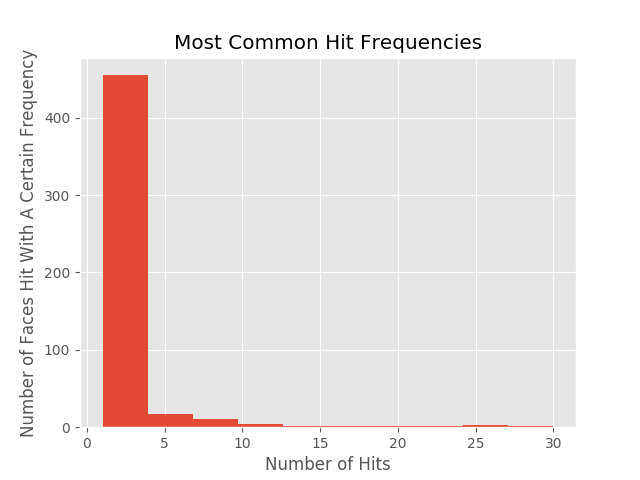
\includegraphics[width=300px]{histogram.png}
		\label{histogram}
		\caption{Frequency With Which Faces of Master Polyhedra are Hit}
	\end{figure}
	
	
	\section{Conclusion}
	We presented an overview of a variety of different methods for enumerating Gomory's Master Corner Polyhedron. These included implementations of algorithms based on ideas from the original paper which utilized the vertex enumeration software contained in the SageMath as well as some simple optimizations which drew upon the symmetries inherited from the group structure. We also examined some approaches which instead of opting for a complete enumeration of the vertices and faces, settled for a partial enumeration.
	In the case of the method based on the Shooting Theorem, this approach exposed some of the faces of groups of order 30, which would have been computationally intractable using other approaches.
	
	The efficient computation of these polyhedra enables the development of stronger cutting plane algorithms since any valid cutting plane inequality for the corner polyhedron will be valid for the integer program associated with the corner polyhedron. The generation of stronger cuts to solve optimization problems on the corner polyhedron itself could also lead to the algorithms which enable solving general integer programs. Creating quick methods for enumerating corner polyhedron would act to aid in future endeavors toward efficiently solving general mixed integer programs.
	
	\bibliographystyle{unsrt}
	\bibliography{project.bib}
	
	\appendix
	\section{Selected Polyhedra with group order $n \le 8$}
	In this section, we compile a subset of the polyhedra which have been computed with groups having order up to at most 8. We have fully enumerated corner polyhedra which have corresponding groups of up to order 20, however these polyhedra have too many faces and vertices to list in their entirety.
	
	We list all faces in the format $b + a_0 + \ldots + a_n = 0$. When we list the incidence matrices, we note that the entry in row $i$ column $j$ being 1 indicates that vertex $i$ is incident to face $j$. We also note that when we write the group $G_{i}$ we mean the cyclic group of order $i$, and when we write $G_{i,j}$ we mean the direct product of the cyclic group of order $i$ with the cyclic group of order $j$. A similar notation holds for products of three or more cyclic groups.
	
	All code and all the master corner polyhedra for groups up to order 20 can be found on \texttt{https://github.com/domyang/cornerpolyhedra}.



\begin{table}[H]
	\centering
	\caption{Faces of $P(G_2, (1))$}
	\label{G2Faces1}
	\begin{tabular}{@{}lll@{}}
		\toprule
		index & b  & a\_0 \\ \midrule
		0     & -1 & 1    \\ \bottomrule
	\end{tabular}
\end{table}

\begin{table}[H]
	\centering
	\caption{Vertices of $P(G_2, (1))$}
	\label{G2Verts1}
	\begin{tabular}{@{}ll@{}}
		\toprule
		Index & t\_0 \\ \midrule
		0     & 1    \\ \bottomrule
	\end{tabular}
\end{table}

\begin{table}[H]
	\centering
	\caption{Incidence Matrix of $P(G_2, (1))$}
	\label{G2Inc1}
	\begin{tabular}{@{}ll@{}}
		\toprule
		& 0 \\ \midrule
		0 & 1 \\ \bottomrule
	\end{tabular}
\end{table}

\begin{table}[H]
	\centering
	\caption{Faces of $P(G_3, (0))$}
	\label{G3Faces}
	\begin{tabular}{@{}llll@{}}
		\toprule
index & b  & a\_0 & a\_1 \\ \midrule
0     & 0  & 0    & 1    \\
1     & 0  & 1    & 0    \\
2     & -3 & 1    & 2    \\
3     & -3 & 2    & 1    \\ \bottomrule
	\end{tabular}
\end{table}

\begin{table}[H]
	\centering
	\caption{Vertices of $P(G_3, (0))$}
	\label{G3Verts}
	\begin{tabular}{@{}lll@{}}
		\toprule
		Index & t\_0 & t\_1 \\ \midrule
		0     & 3    & 0    \\
		1     & 1    & 1    \\
		2     & 0    & 3    \\ \bottomrule
	\end{tabular}
\end{table}

\begin{table}[H]
	\centering
	\caption{Incidence Matrix of $P(G_3, (0))$}
	\label{G3Inc}
	\begin{tabular}{@{}lllll@{}}
		\toprule
		& 0 & 1 & 2 & 3 \\ \midrule
		0 & 1 & 0 & 1 & 0 \\
		1 & 0 & 0 & 1 & 1 \\
		2 & 0 & 1 & 0 & 1 \\ \bottomrule
	\end{tabular}
\end{table}

\begin{table}[H]
	\centering
	\caption{Faces of $P(G_3, (2))$}
	\label{G3Faces2}
	\begin{tabular}{@{}llll@{}}
		\toprule
		index & b  & a\_0 & a\_1 \\ \midrule
		0     & 0  & 0    & 1    \\
		1     & 0  & 1    & 0    \\
		2     & -2 & 1    & 2    \\ \bottomrule
	\end{tabular}
\end{table}

\begin{table}[H]
	\centering
	\caption{Vertices of $P(G_3, (2))$}
	\label{G3Verts2}
	\begin{tabular}{@{}lll@{}}
		\toprule
		Index & t\_0 & t\_1 \\ \midrule
		0     & 0    & 1    \\
		1     & 2    & 0    \\ \bottomrule
	\end{tabular}
\end{table}

\begin{table}[H]
	\centering
	\caption{Incidence Matrix of $P(G_3, (2))$}
	\label{G3Inc2}
	\begin{tabular}{@{}llll@{}}
		\toprule
		& 0 & 1 & 2 \\ \midrule
		0 & 0 & 1 & 1 \\
		1 & 1 & 0 & 1 \\ \bottomrule
	\end{tabular}
\end{table}

\begin{table}[H]
	\centering
	\caption{Faces of $P(G_{2,2}, (0,0))$}
	\label{G22Faces}
	\begin{tabular}{@{}lllll@{}}
		\toprule
		index & b  & a\_0 & a\_1 & a\_2 \\ \midrule
		0     & 0  & 0    & 0    & 1    \\
		1     & 0  & 0    & 1    & 0    \\
		2     & 0  & 1    & 0    & 0    \\
		3     & -2 & 1    & 1    & 1    \\ \bottomrule
	\end{tabular}
\end{table}

\begin{table}[H]
	\centering
	\caption{Vertices of $P(G_{2,2}, (0,0))$}
	\label{G22Verts}
	\begin{tabular}{@{}llll@{}}
		\toprule
		Index & t\_0 & t\_1 & t\_2 \\ \midrule
		0     & 0    & 0    & 2    \\
		1     & 2    & 0    & 0    \\
		2     & 0    & 2    & 0    \\ \bottomrule
	\end{tabular}
\end{table}

\begin{table}[H]
	\centering
	\caption{Incidence Matrix of $P(G_{2,2}, (0, 0))$}
	\label{G22Inc}
	\begin{tabular}{@{}lllll@{}}
		\toprule
		& 0 & 1 & 2 & 3 \\ \midrule
		0 & 0 & 1 & 1 & 1 \\
		1 & 1 & 1 & 0 & 1 \\
		2 & 1 & 0 & 1 & 1 \\ \bottomrule
	\end{tabular}
\end{table}

\begin{table}[H]
	\centering
	\caption{Faces of $P(G_6, (0))$}
	\label{G6Faces}
	\begin{tabular}{@{}lllllll@{}}
		\toprule
		index & b  & a\_0 & a\_1 & a\_2 & a\_3 & a\_4 \\ \midrule
		0     & 0  & 0    & 0    & 0    & 0    & 1    \\
		1     & 0  & 0    & 0    & 0    & 1    & 0    \\
		2     & 0  & 0    & 0    & 1    & 0    & 0    \\
		3     & 0  & 0    & 1    & 0    & 0    & 0    \\
		4     & 0  & 1    & 0    & 0    & 0    & 0    \\
		5     & -6 & 2    & 3    & 4    & 2    & 4    \\
		6     & -6 & 2    & 3    & 4    & 5    & 1    \\
		7     & -6 & 4    & 3    & 2    & 1    & 5    \\
		8     & -6 & 4    & 3    & 2    & 4    & 2    \\ \bottomrule
	\end{tabular}
\end{table}

\begin{table}[H]
	\centering
	\caption{Vertices of $P(G_6, (0))$}
	\label{G6Verts}
	\begin{tabular}{@{}llllll@{}}
		\toprule
		Index & t\_0 & t\_1 & t\_2 & t\_3 & t\_4 \\ \midrule
		0     & 0    & 2    & 0    & 0    & 0    \\
		1     & 0    & 0    & 0    & 1    & 1    \\
		2     & 0    & 0    & 3    & 0    & 0    \\
		3     & 1    & 0    & 1    & 0    & 0    \\
		4     & 3    & 0    & 0    & 0    & 0    \\
		5     & 0    & 0    & 0    & 0    & 6    \\
		6     & 1    & 0    & 0    & 2    & 0    \\
		7     & 0    & 0    & 0    & 6    & 0    \\
		8     & 0    & 0    & 1    & 0    & 2    \\ \bottomrule
	\end{tabular}
\end{table}

\begin{table}[]
	\centering
	\caption{Incidence Matrix of $P(G_6, (0))$}
	\label{G6Inc}
	\begin{tabular}{@{}llllllllll@{}}
		\toprule
		& 0 & 1 & 2 & 3 & 4 & 5 & 6 & 7 & 8 \\ \midrule
		0 & 1 & 1 & 1 & 0 & 1 & 1 & 1 & 1 & 1 \\
		1 & 0 & 0 & 1 & 1 & 1 & 1 & 1 & 1 & 1 \\
		2 & 1 & 1 & 0 & 1 & 1 & 0 & 0 & 1 & 1 \\
		3 & 1 & 1 & 0 & 1 & 0 & 1 & 1 & 1 & 1 \\
		4 & 1 & 1 & 1 & 1 & 0 & 1 & 1 & 0 & 0 \\
		5 & 0 & 1 & 1 & 1 & 1 & 0 & 1 & 0 & 0 \\
		6 & 1 & 0 & 1 & 1 & 0 & 1 & 0 & 1 & 0 \\
		7 & 1 & 0 & 1 & 1 & 1 & 0 & 0 & 1 & 0 \\
		8 & 0 & 1 & 0 & 1 & 1 & 0 & 1 & 0 & 1 \\ \bottomrule
	\end{tabular}
\end{table}

\begin{table}[H]
	\centering
	\caption{Faces of $P(G_{2,2,2}, (0,0,0))$}
	\label{G222Faces}
	\begin{tabular}{@{}lllllllll@{}}
		\toprule
		index & b  & a\_0 & a\_1 & a\_2 & a\_3 & a\_4 & a\_5 & a\_6 \\ \midrule
		0     & 0  & 0    & 0    & 0    & 0    & 0    & 0    & 1    \\
		1     & 0  & 0    & 0    & 0    & 0    & 0    & 1    & 0    \\
		2     & 0  & 0    & 0    & 0    & 0    & 1    & 0    & 0    \\
		3     & 0  & 0    & 0    & 0    & 1    & 0    & 0    & 0    \\
		4     & 0  & 0    & 0    & 1    & 0    & 0    & 0    & 0    \\
		5     & 0  & 0    & 1    & 0    & 0    & 0    & 0    & 0    \\
		6     & 0  & 1    & 0    & 0    & 0    & 0    & 0    & 0    \\
		7     & -2 & 1    & 1    & 1    & 1    & 1    & 1    & 1    \\ \bottomrule
	\end{tabular}
\end{table}

\begin{table}[H]
	\centering
	\caption{Vertices of $P(G_{2,2,2}, (0,0,0))$}
	\label{G222Vert}
	\begin{tabular}{@{}llllllll@{}}
		\toprule
		Index & t\_0 & t\_1 & t\_2 & t\_3 & t\_4 & t\_5 & t\_6 \\ \midrule
		0     & 0    & 0    & 0    & 0    & 0    & 0    & 2    \\
		1     & 2    & 0    & 0    & 0    & 0    & 0    & 0    \\
		2     & 0    & 2    & 0    & 0    & 0    & 0    & 0    \\
		3     & 0    & 0    & 2    & 0    & 0    & 0    & 0    \\
		4     & 0    & 0    & 0    & 2    & 0    & 0    & 0    \\
		5     & 0    & 0    & 0    & 0    & 2    & 0    & 0    \\
		6     & 0    & 0    & 0    & 0    & 0    & 2    & 0    \\ \bottomrule
	\end{tabular}
\end{table}

\begin{table}[H]
	\centering
	\caption{Incidence Matrix of $P(G_{2,2,2}, (0,0,0))$}
	\label{G222Inc}
	\begin{tabular}{@{}lllllllll@{}}
		\toprule
		& 0 & 1 & 2 & 3 & 4 & 5 & 6 & 7 \\ \midrule
		0 & 0 & 1 & 1 & 1 & 1 & 1 & 1 & 1 \\
		1 & 1 & 1 & 1 & 1 & 1 & 1 & 0 & 1 \\
		2 & 1 & 1 & 1 & 1 & 1 & 0 & 1 & 1 \\
		3 & 1 & 1 & 1 & 1 & 0 & 1 & 1 & 1 \\
		4 & 1 & 1 & 1 & 0 & 1 & 1 & 1 & 1 \\
		5 & 1 & 1 & 0 & 1 & 1 & 1 & 1 & 1 \\
		6 & 1 & 0 & 1 & 1 & 1 & 1 & 1 & 1 \\ \bottomrule
	\end{tabular}
\end{table}

\end{document}